%!TEX root = paper.tex
%%%%%%%%%%%%%%%%%%%%%%%%%%%%%%%%%%%%%%%%%%%%%%%%%%%%%%%%%%%%%%%%%%%%%%%%%%%%%%%%
\section{Quality Model, Mappings and Map}
\label{sec:qoe}

Speaking of community maps, this bring us to the final tasks of interpreting the collected data as YouTube quality and presenting it in an easy-to-grasp way to the community. As discussed in Section~\ref{sec:relatedwork} there do exists metrics that derive a higher layer abstraction from directly measurable values, such as the bitrate. E.g. \cite{hossfeld2011transport} fitted the \textbf{stalling frequency} $F$ from throughput samples as

\begin{equation*}
F(X) = -1.09 e^{-1.18 \frac{V}{B}} + 0.36
\end{equation*}

for transmission bandwidths $B$ and video bitrates $V$. But a stalling frequency is nothing that can be easily understood in terms of YouTube quality by the community, and therefore a simpler metric is desired. For this let's consider the \textbf{reception rate} $\rho = \frac{B}{V}$ \cite{Hossfeld2013}. This means that as long as the transmission rate is above the video rate the video streaming should work well, bar any variations. This is even more so if you include a safety margin as evaluated in, e.g., \cite{Zinner2015}. A \SI{25}{\percent} surplus of the transmission rate should therefore take care of this and ensure the video to be playable at the selected quality level at all times. This then yields a definition of the playable video quality $v_{playable}$ for our system as

\begin{equation*}
\phantom{\text{.}} v_{playable} = \max\left(\left\{ v | v \in \mathbb{V} \wedge 1.25 \cdot v < B \right\}\right) \text{.}
\end{equation*}

Used as the set of $V$ is here simply YouTube's recommended video encoding bitrates\footnote{Based on information from \url{https://support.google.com/youtube/answer/1722171?hl=en}. Do note that these are recommendations for the video upload before they are transcoded by YouTube. But this gives a rough estimate for the download bitrate as well.} as listed in Table~\ref{tab:recvidbr}.

\begin{table}[!t]
	\caption{Recommended YouTube video bitrates for 30 fps video, mean stalling frequency, and ratio of bandwidth samples above $1.25 \times V$ in the measurement data.}
	\label{tab:recvidbr}
	\begin{tabu}{XSSS}
	\toprule
	\textbf{Res.} & {\textbf{Video Bitrate}} & {\textbf{Stalling Frequency}} & {\textbf{Ratio of} $\mathbf{B}$} \\
	& {$\mathbf{V}$ (\textbf{\si{\mega\bit\per\second})}} & $\mathbf{F}$ & {\textbf{above} $\mathbf{1.25 \times V}$} \\
	\midrule
	\textbf{2160p} & 45 & 0.35 & 0 \\
	\textbf{1440p} & 16 & 0.23 & 0 \\
	\textbf{1080p} & 8 & 0.09 & 0.34 \\
	\textbf{720p} & 5 & 0.04 & 0.67 \\
	\textbf{480p} & 2.5 & 0.01 & 0.90 \\
	\textbf{360p} & 1 & 0.00 & 0.98 \\
	\bottomrule
	\end{tabu}
\end{table}

\begin{figure}[!t]
    \centering
    \begin{subfigure}[b]{0.45\columnwidth}
        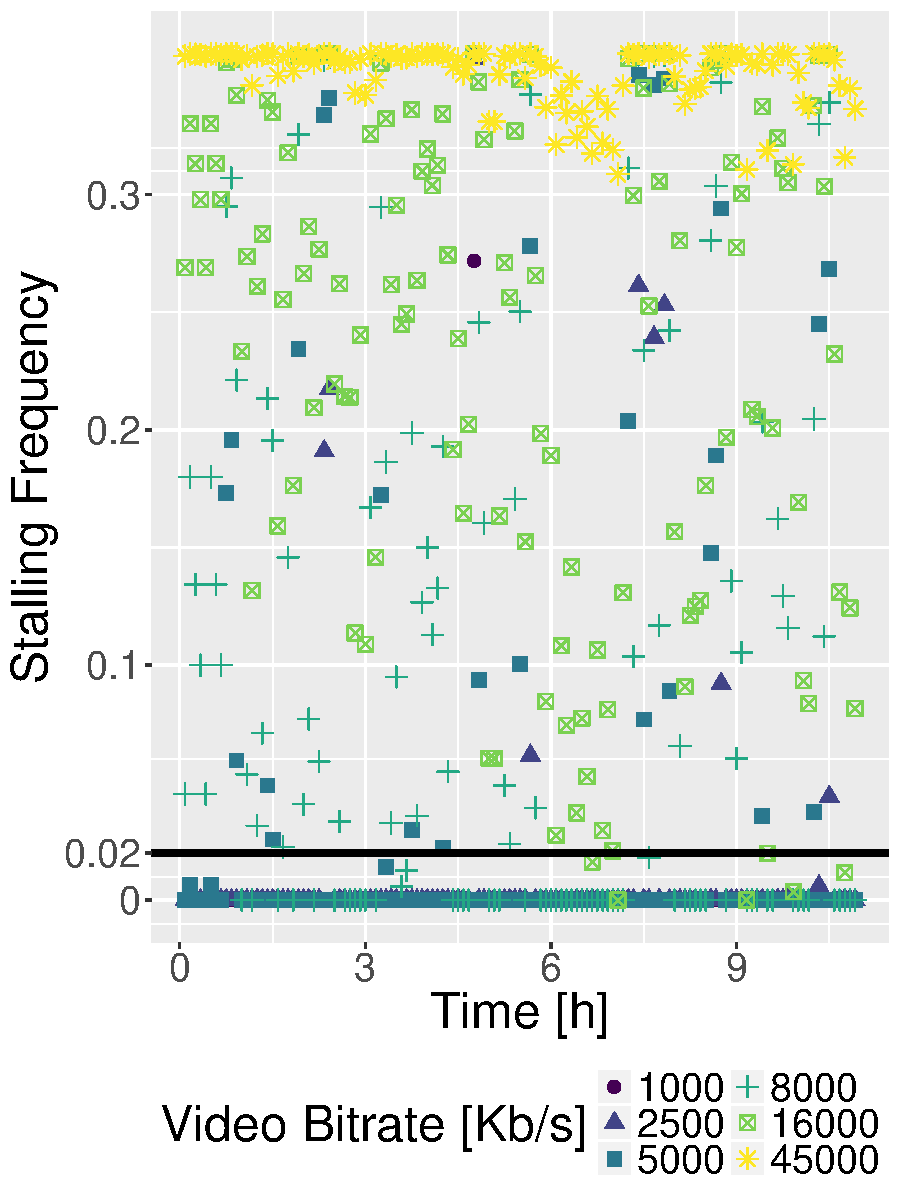
\includegraphics[width=\textwidth]{images/stallingfreq-timeseries.pdf}
        \caption{Stalling frequency (according to \cite{hossfeld2011transport}) time series.}
        \label{fig:stallingfreq}
    \end{subfigure}
    ~
    \begin{subfigure}[b]{0.45\columnwidth}
        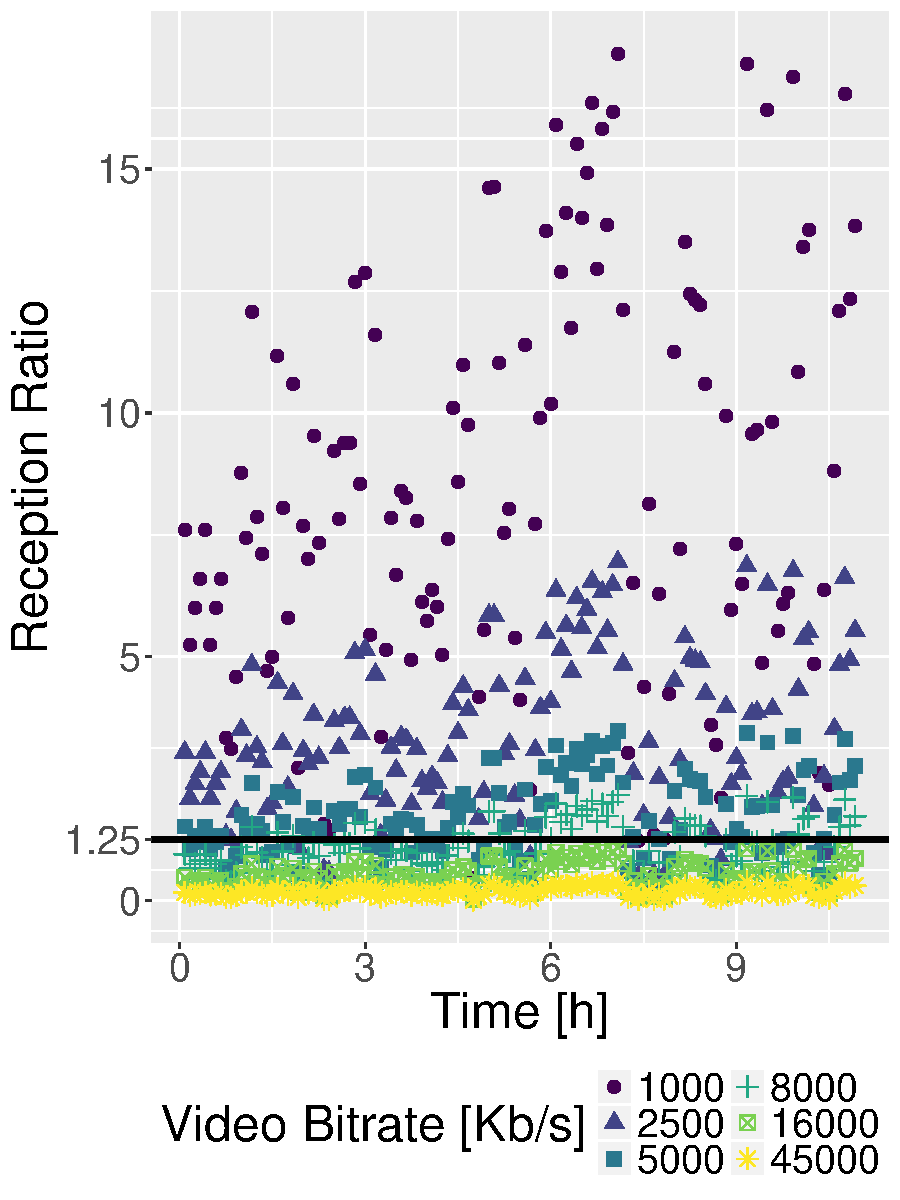
\includegraphics[width=\textwidth]{images/receptionratio-timeseries.pdf}
        \caption{Reception ratio (according to \cite{Hossfeld2013}) time series.}
        \label{fig:receptionratio}
    \end{subfigure}

    \begin{subfigure}[b]{0.45\columnwidth}
        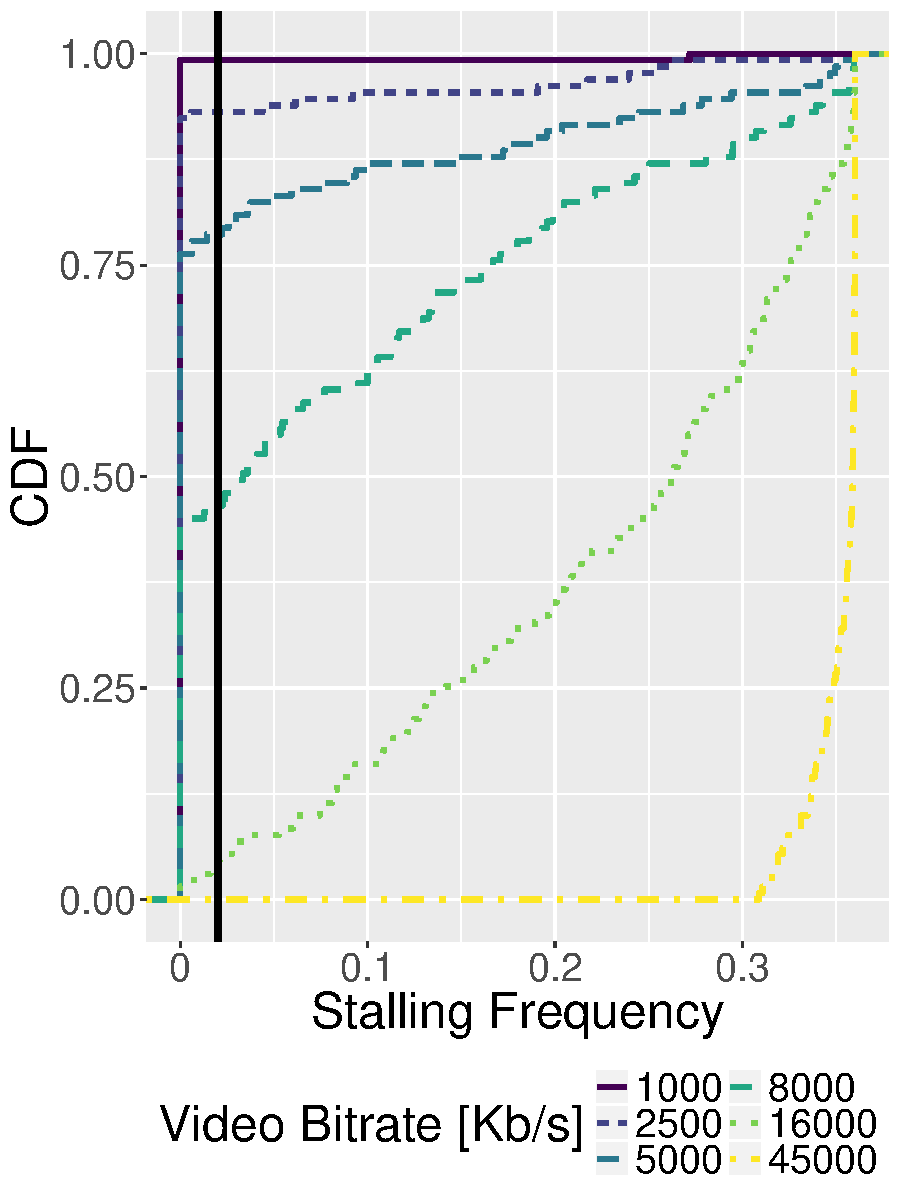
\includegraphics[width=\textwidth]{images/stallingfreq-cdf.pdf}
        \caption{Corresponding CDF of the stalling frequency.}
        \label{fig:stallingfreq-cdf}
    \end{subfigure}
    ~
    \begin{subfigure}[b]{0.45\columnwidth}
        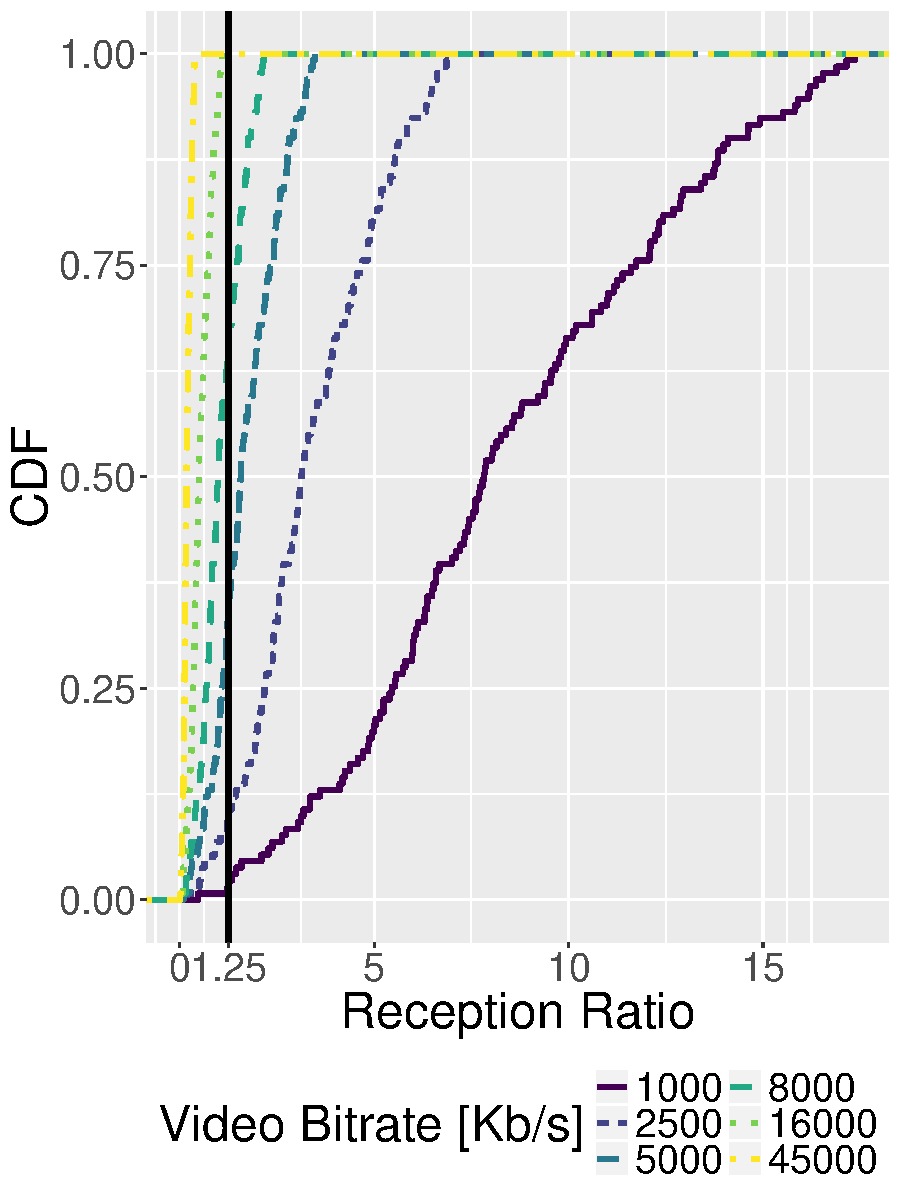
\includegraphics[width=\textwidth]{images/receptionratio-cdf.pdf}
        \caption{Corresponding CDF of the reception ratio.}
        \label{fig:receptionratio-cdf}
    \end{subfigure}
    \caption{Time series and \acrshort{CDF} depictions of the two derived video streaming quality metrics, matching the throughput to the desired video video bitrate. Horizontal --- respectively vertical --- lines denote the selected cutoff threshold for an acceptable streaming quality.}
    \label{fig:timeseries}
\end{figure}

Each spatial region now has to have a series of bandwidth samples attached to it, taken at different points of time. Figure~\ref{fig:timeseries} demonstrates such a time series for one location as both the stalling frequency and the reception rate with the discussed threshold of $1.25$. This also clearly demonstrates large temporal fluctuations for the playable video quality, which should also be exposed in the community quality map, e.g. through some additional, advanced information overlays for each location. Yet, the default geographical map should be kept free of such temporal data to avoid overwhelming the users.

In order to provide a clutter-free representation the mapping service needs to decide for just one specific video quality rating at each location. This requires some form of temporal averaging to be conducted. Here, the system will color the map in the highest video quality of which \SI{90}{\percent} of the bandwidth samples over the measured period were above $1.25 \times V$.

Both the more complex stalling frequency --- using a similar threshold of \SI{2}{\percent} here --- and the reception ratio representation result in the same quality decisions here. Moreover, the two metrics have a Pearson correlation coefficient of $-0.92$. This means that even this simple metric is sufficiently able to visualize the service's quality, and no more complex metric needs to be employed here. With this, the results also become easily comparable to other approaches  (e.g. YouSlow\cite{Nam:2014:YPA:2619239.2631433}) that rely on directly measuring the rebuffering rate (which is akin to the stalling frequency $F$). A mockup of the resulting geographical map and video quality overlay is shown in Figure~\ref{fig:videoquality-map}. Common caveats of geographical grouping and interpolation of samples also apply to this type of video quality map and still need to be solved.

\begin{figure}[!t]
	\centering
	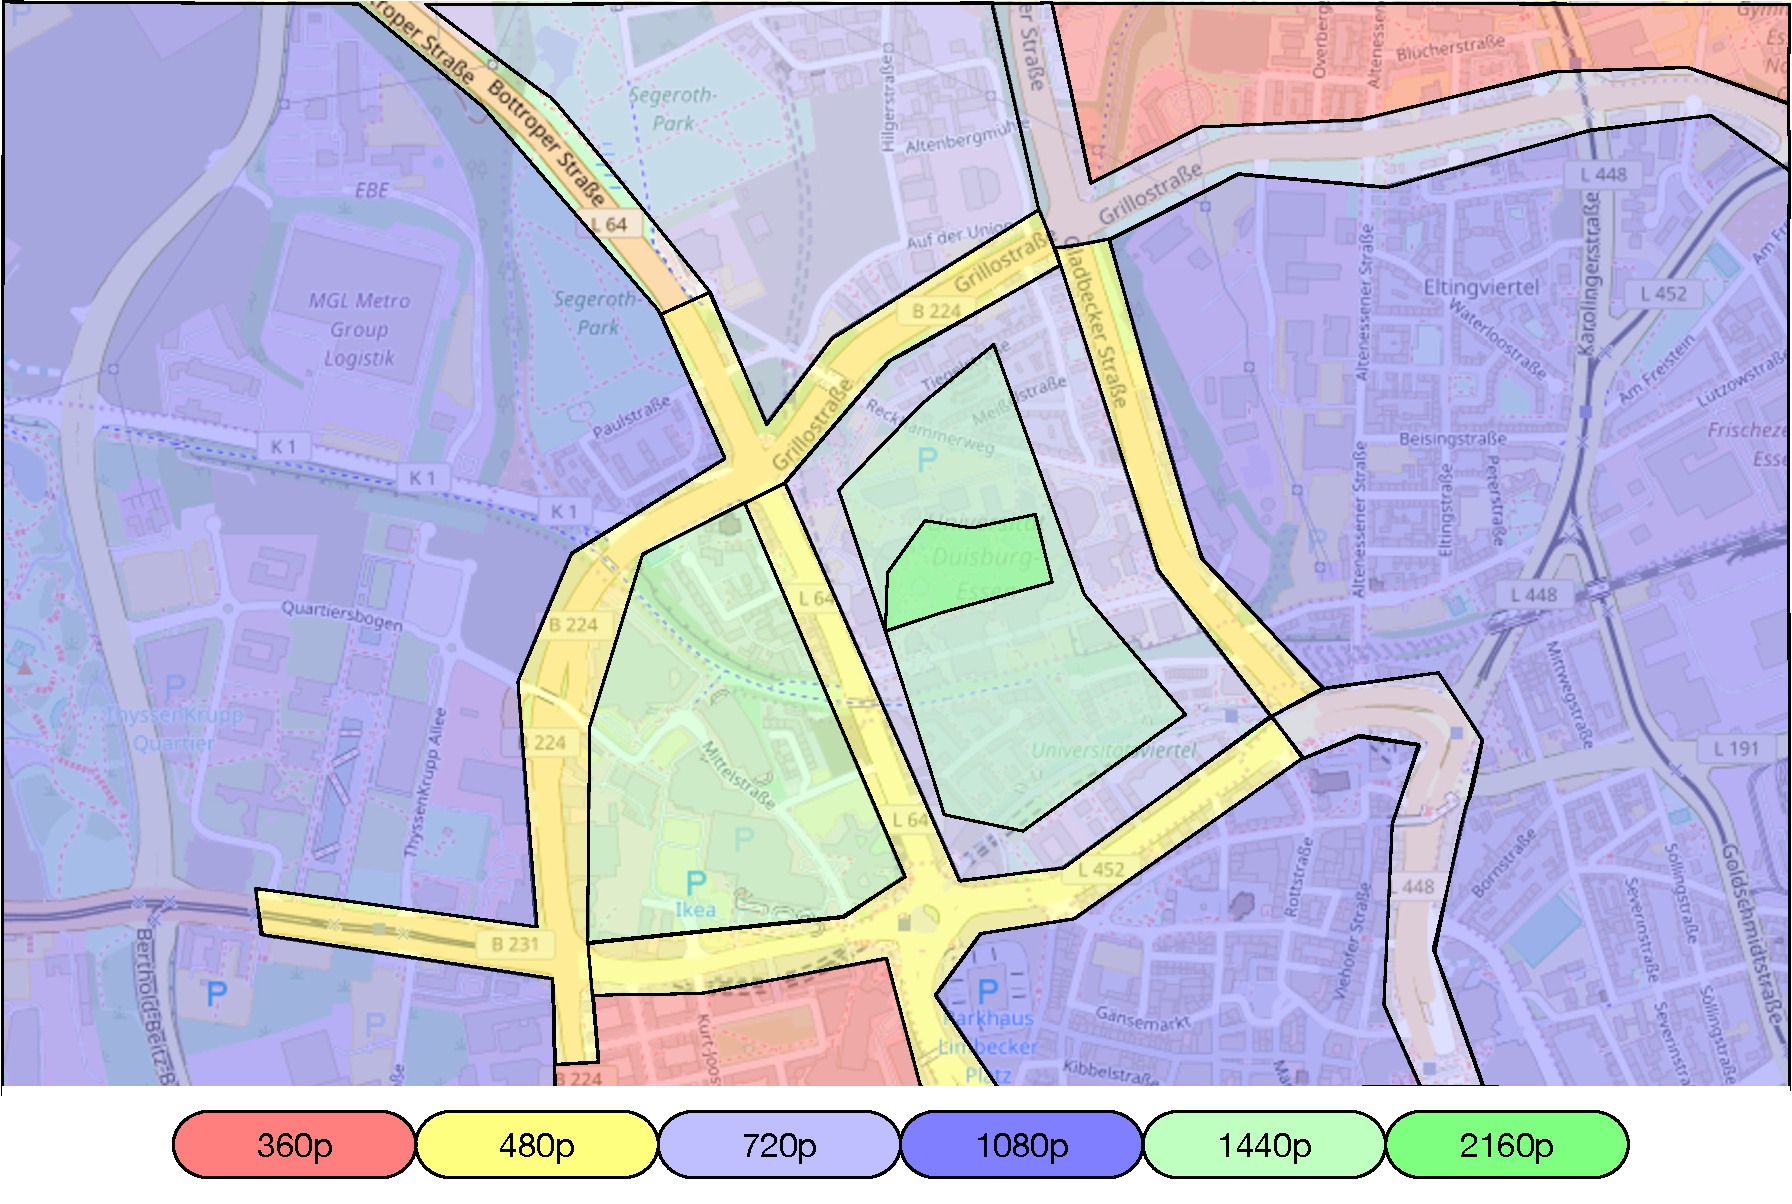
\includegraphics[width=1.0\columnwidth]{images/qoe-map-mockup.pdf}
	\caption{Mockup map of achievable YouTube video resolution for specific regions for a mobile provider. Regions should be grouped and interpolated from individual participants' measurements.}
\label{fig:videoquality-map}
\end{figure}


Now consider this map for a hypothetical use case of someone having to move to a new place. It is common today to check the new apartment's location for good internet access, both wired as well as mobile. Using our approach that person would then not just be able to tell if there is connectivity in that area --- as in most other participatory sensing approaches --- but also if a specific service works in an acceptable quality there, especially at the time of day when one is at home.

While YouTube does serve as the example here, it is important to note that, with the available throughput data, similar mappings and visualizations can easily be achieved for any other kind of service. This is just a matter of switching the mapping function to another, appropriate one for that service. This would allow the community crowdsensed map to be easily extensible and able to be personalized to show the quality of one's favorite services. All while still avoiding to collect resource-intense service-specific data and therefore able to easily scaled up to a large community.
